% Standalone source for Figure 4 (the ying->three_gorges corridor).
% Reproduce:  pdflatex figures/corridor.tex   (produces figures/corridor.pdf)
% Node-link schematic built from the engine topology (src/engine/topology.py).
\documentclass[border=3pt]{standalone}
\usepackage{tikz}
\usetikzlibrary{positioning}
\begin{document}
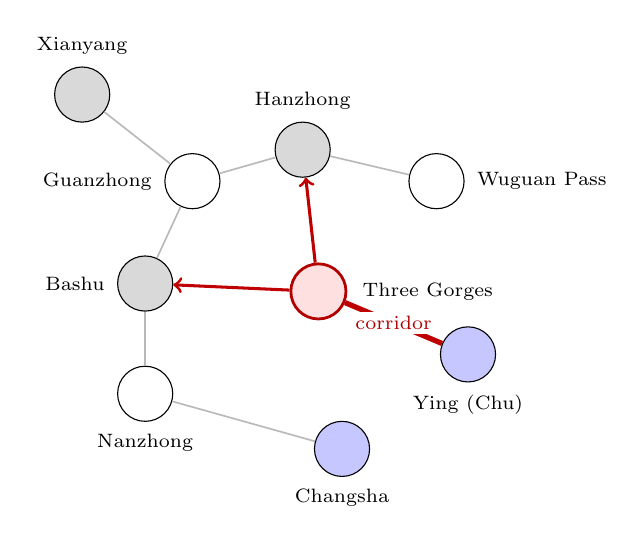
\begin{tikzpicture}[
  font=\small,
  sc/.style={circle,draw,minimum size=7mm,inner sep=1pt,line width=0.4pt},
  qin/.style={sc,fill=gray!30},
  chu/.style={sc,fill=blue!22},
  neu/.style={sc,fill=white},
  choke/.style={sc,fill=red!12,line width=1pt,draw=red!70!black},
  edge/.style={gray!55,line width=0.6pt},
  strike/.style={red!75!black,line width=1.1pt,->},
  corridor/.style={red!75!black,line width=1.9pt},
  lbl/.style={font=\scriptsize}
]
\node[qin]   (xian) at (0,4)    {}; \node[lbl,above=1pt of xian]  {Xianyang};
\node[neu]   (guan) at (1.4,2.9) {}; \node[lbl,left=1pt of guan]  {Guanzhong};
\node[qin]   (hanz) at (2.8,3.3) {}; \node[lbl,above=1pt of hanz] {Hanzhong};
\node[neu]   (wugu) at (4.5,2.9) {}; \node[lbl,right=1pt of wugu] {Wuguan Pass};
\node[qin]   (bash) at (0.8,1.6) {}; \node[lbl,left=1pt of bash]  {Bashu};
\node[neu]   (nanz) at (0.8,0.2) {}; \node[lbl,below=1pt of nanz] {Nanzhong};
\node[choke] (tg)   at (3.0,1.5) {}; \node[lbl,right=2pt of tg]   {Three Gorges};
\node[chu]   (ying) at (4.9,0.7) {}; \node[lbl,below=1pt of ying] {Ying (Chu)};
\node[chu]   (chan) at (3.3,-0.5){}; \node[lbl,below=1pt of chan] {Changsha};
\draw[edge] (xian)--(guan); \draw[edge] (guan)--(hanz); \draw[edge] (guan)--(bash);
\draw[edge] (hanz)--(wugu); \draw[edge] (bash)--(nanz); \draw[edge] (nanz)--(chan);
\draw[strike] (tg)--(hanz); \draw[strike] (tg)--(bash);
\draw[corridor] (ying)--(tg) node[midway,fill=white,inner sep=1.5pt,lbl,text=red!70!black]{corridor};
\end{tikzpicture}
\end{document}
